%% CHAPTER HEADER ////////////////////////////////////////////////////////////////////////////////
\chapter[Deep learning for SHM]{Deep learning approaches for SHM}
\label{ch3}
%% CHAPTER INTRODUCTION ///////////////////////////////////////////////////////////////////////////////
%%%%%%%%%%%%%%%%%%%%%%%%%%%%%%%%%%%%%%%%%%%%%%%%%%%%%%%%%%%%%%%%%%%%%%%%%%%%%%%%
Artificial Intelligence (AI) refers to the ability of machines to imitate the human mind in such a way as  \enquote{learning and problem-solving}~\cite{Russell2010}.
AI has various definitions, however, it can be defined as any device that can sense its environment and consequently takes steps that maximize its opportunity of accomplishing its goals~\cite{Russell2010}.
Historically, AI was introduced in 1956 at the Dartmouth summer conference by John McCarthy.
For many years after Dartmouth summer conference, AI has been in \enquote{AI winter} due to the lack of computational power.
Moreover, its algorithms were not fully understood mathematically.
However, in recent years, AI has returned to the stage due to several reasons. 
The first reason was the advanced evolution that occurred in technology that produced high computational powers (e.g. Graphics Processing Unit (GPU)). 
GPU computational power exceeds the traditional Central Processing Units (CPUs) due to the high capability of parallel computing, which makes it more efficient in running algorithms for large data.
The second reason is the tremendous data available nowadays, which can remarkably improve the learning process of an AI system, as its effectiveness depends on learning from its environment. 

In general, AI can be divided into two classes: Strong AI and weak AI. Tab.~\ref{tab:Strong_Weak_AI} presents the main differences between them.
%%%%%%%%%%%%%%%%%%%%%%%%%%%%%%%%%%%%%%%%%%%%%%%%%%%%%%%%%%%%%%%%%%%%%%%%%%%%%%%%
\begin{table}[h]
	\renewcommand{\arraystretch}{1.1}
	\centering
	\caption{AI classes}
	\scriptsize
	\begin{tabular}{p{2cm}p{4cm}p{4cm}} 
		\toprule
		\textbf{Category} & \textbf{Strong AI} & \textbf{Weak AI} \\ \midrule
		\textbf{Definition} & Sort of AI that possesses the same human intellectual capabilities, or exceeds it. & Sort of AI that is utilised for a specific application design. \\ \midrule
		
		\textbf{Purpose} &To surpass and replace the human mind  &  To imitate the human intellectual thinking. \\  
		\bottomrule
	\end{tabular}
	\label{tab:Strong_Weak_AI}
\end{table}
%%%%%%%%%%%%%%%%%%%%%%%%%%%%%%%%%%%%%%%%%%%%%%%%%%%%%%%%%%%%%%%%%%%%%%%%%%%%%%%%
\paragraph{}
Engineering structures such as buildings, roads, tunnels, power generation systems, rotating machinery, and aircraft are considered important in our modern life.
However, such structures are prone to various types of damage.
Therefore, it is essential to maintain them and keep them safe during their operational lifetime.
Health monitoring presents an essential tool in management activities as it allows identifying early and progressive structural damage~\cite{Farrar2007}. 
Obtained data from monitoring structures are large and need to be transformed into valuable information to assist the development and design of maintenance activities, improve safety, reduce uncertainties and extend our knowledge regarding the monitored structure.

SHM is one of the most robust tools for managing infrastructure.
Traditionally, the procedure of performing an autonomous damage identification for engineering structures, such as civil, mechanical or aerospace, is referred to as SHM~\cite{farrar2001vibration}.
SHM aims to describe a real-time evaluation of a structure during its life-cycle~\cite{Balageas2010}. 
Moreover, SHM assists in detecting and characterizing damage in a structure as a whole or its parts. 
Damage detection in a structure is crucial since it may reduce safety and performance during its operational lifetime~\cite{Yuan2016}.
Furthermore, the SHM approach involves monitoring a structure continuously through an array of sensors that periodically measure the response of the structure, then extracting the sensitive damage features from these measurements to perform statistical analysis on these features to examine the condition of the structure.

Generally, there are two approaches to SHM: physics-based and
data-based.
In the physics-based approach, the inverse problem method is applied in which numerical models such as finite element models are implemented. 
Damage identification results by comparing the registered readings from the structure and the estimated data from the models.
On the other hand, the data-based approach is related to the AI domain (machine learning and deep learning), in which models are developed to learn the behavior of the structure based on earlier registered data that leads to performing pattern recognition for the damage identification.

The data-based approach can be applied for both supervised and unsupervised learning~\cite{worden2007application}.
Supervised learning can be utilised in the field of SHM, where data of the damaged and undamaged conditions are available in which the detection models can train~\cite{figueiredo2018machine}.
On the other hand, unsupervised learning is applied when data of undamaged cases are only available.
Therefore, the detection models train only on such data~\cite{figueiredo2018machine}.

%% INCLUDE SECTIONS ///////////////////////////////////////////////////////////////////////////////////

%%%%%%%%%%%%%%%%%%%%%%%%%%%%%%%%%%%%%%%%%%%%%%%%%%%%%%%%%%%%%%%%%%%%%%%%%%%%%%%%
\section{Machine learning approach}
\label{sec31}
%%%%%%%%%%%%%%%%%%%%%%%%%%%%%%%%%%%%%%%%%%%%%%%%%%%%%%%%%%%%%%%%%%%%%%%%%%%%%%%%
Machine learning (ML) is a sub-field of AI which belongs to the computer science field. 
ML is defined as \enquote{the ability of a computer to learn without being explicitly programmed}~\cite{munoz2014machine}.

The conventional way of software engineering is by creating rules by humans and combining them with data to create a solution to a problem.
Alternatively, when it comes to ML, it utilises data and answers to learn the rules behind the problem~\cite{franoischollet2017learning}.
In Fig.~\ref{fig:Machine_learning} the conventional software programming and ML are presented in (a) and (b) respectively.
In ML, machines have to run into a learning process to learn inference rules, which are responsible for controlling the relations within a phenomenon. Hence, it is called an ML.
%%%%%%%%%%%%%%%%%%%%%%%%%%%%%%%%%%%%%%%%%%%%%%%%%%%%%%%%%%%%%%%%%%%%%%%%%%%%%%%%
\begin{figure} [!ht]
	\begin{center}
		\centering
		\includegraphics[scale=1]{Figures/Chapter_1/machine_learning_vs_conventional_programming.png}
	\end{center}
	\caption{(a) Conventional Programming	(b) Machine learning} 
	\label{fig:Machine_learning}
\end{figure}
%%%%%%%%%%%%%%%%%%%%%%%%%%%%%%%%%%%%%%%%%%%%%%%%%%%%%%%%%%%%%%%%%%%%%%%%%%%%%%%%
\paragraph{}
ML techniques in SHM were heavily utilised by researchers for damage detection~\cite{raghavan2008effects, Su2009, Mitra2016}.
Moreover, ML techniques attempt to map the patterns of the input data acquired by sensors to output targets for a damage estimation at different levels. 
Accordingly, ML techniques demand high domain knowledge of the examiner to perform hand-crafted damage-sensitive feature extraction on the raw data acquired by sensors before being fed into a suitable ML model.
Generally, the process of damage-sensitive features extraction (hand-crafted) in the field of SHM emerged due to the enormous development in the physics-based SHM techniques such as modal strain energy (MSE)~\cite{Kim}, modal curvature (MC)~\cite{Wahab}, modal assurance criterion (MAC), and Coordinate (MAC)~\cite{Allemang2003}, modal flexibility (MF)~\cite{Jaishi}, damage locating vector (DLV)~\cite{Bernal2002}, wavelet transform~\cite{Staszewski,Kima} and probabilistic reconstruction algorithm (PRA)~\cite{Hay2006} among others.
%%%%%%%%%%%%%%%%%%%%%%%%%%%%%%%%%%%%%%%%%%%%%%%%%%%%%%%%%%%%%%%%%%%%%%%%%%%%%%%%

Different methods can be implemented when performing ML. 
Generally, those methods are grouped into four approaches: Supervised learning, Unsupervised learning, Reinforcement learning, and Transfer learning approach.
Fig.~\ref{fig:Machine_learning_approaches} shows the different types of ML approaches.
%%%%%%%%%%%%%%%%%%%%%%%%%%%%%%%%%%%%%%%%%%%%%%%%%%%%%%%%%%%%%%%%%%%%%%%%%%%%%%%%
\begin{figure} [!ht]
	\begin{center}
		\centering
		\includegraphics[scale=1]{Figures/Chapter_1/ML_approaches.png}
	\end{center}
	\caption{Machine Learning Approaches} 
	\label{fig:Machine_learning_approaches}
\end{figure}
%%%%%%%%%%%%%%%%%%%%%%%%%%%%%%%%%%%%%%%%%%%%%%%%%%%%%%%%%%%%%%%%%%%%%%%%%%%%%%%%
\paragraph{}
Supervised learning is the task of training a machine how to develop inference rules from the training data, and how to map inputs with outputs.
The training data is a collection of variables together with its labels (e.g. a set of civil images) of structures that are labelled as cracked or undamaged (healthy).
During the learning process, the machine gets a collection of inputs simultaneously with the corresponding label (ground truth).
Accordingly, by comparing its predicted output with the correct output to find errors, it modifies the model and the learning occurs~\cite{Ongsulee2018}. 
Supervised learning uses patterns to predict the values of the output label for new unlabeled data by applying methods like regression and classification~\cite{Ongsulee2018}. 
%Fig~\ref{fig:Machine_learning_approaches} presents most utilised algorithms for ML different approaches like: 
%K Nearest Neighbors algorithm (KNN) where K represents the number of the nearest neighbours used for classification of the observations in a test sample, based on their characteristics e.g. the mean distance. 
%Moreover,Decision Trees where the data keeps splitting according to a specific parameter. 
%Furthermore, Naive Bayes algorithm which is based on probabilistic approach, through implementing Bayes' theorem.
%In addition, Support vector Machine SVM and Logistic regression. 
%For Regression purposes, algorithms like linear and polynomial regression are implemented.

Unsupervised Learning is applied to such data with no historical labels~\cite{Ongsulee2018}. 
In this case, the model does not know the ground truth labels of the input values. Therefore, the algorithm needs to figure out some common characteristics among the input values.
Consequently, unsupervised learning is more difficult than supervised learning, due to removing the supervision which implies the problem becomes less defined.
%The most well-known techniques used in Unsupervised learning is clustering~\cite{Russell2010}. 
%In which it creates subgroups within the input data based on their characteristics, Fig~\ref{fig:Machine_learning_approaches} presents most Clustering algorithms like:k-means algorithm, which intends to split n observations into k clusters, where each observation relates to the cluster that has the nearest mean distance.   

Reinforcement learning is based on the trial and error principle, which means the algorithm learns through actions that explore the environment in a way that results in the greatest rewards~\cite{Russell2010}.
In this approach of learning, the process consists of three parts: the agent, which is responsible for making decisions, the environment that relates to any interaction with the agent, and the actions that are made by the agent. Figure.~\ref{fig:ReinforcementLearning} illustrates the procedure of the reinforcement learning approach.
%%%%%%%%%%%%%%%%%%%%%%%%%%%%%%%%%%%%%%%%%%%%%%%%%%%%%%%%%%%%%%%%%%%%%%%%%%%%%%%%
\begin{figure} [!ht]
	\begin{center}
		\centering
		\includegraphics[scale=1]{Figures/Chapter_1/Reinforcement_learning.png}
	\end{center}
	\caption{Reinforcement Learning} 
	\label{fig:ReinforcementLearning}
\end{figure}
%%%%%%%%%%%%%%%%%%%%%%%%%%%%%%%%%%%%%%%%%%%%%%%%%%%%%%%%%%%%%%%%%%%%%%%%%%%%%%%%

Transfer learning differs compared to the traditional ML approaches that are designed for particular tasks, which means their learning, and knowledge can not be transferred from one model to another.
Therefore, when starting a new ML task, we have to start from scratch.
On the contrary, in transfer learning, the model knowledge (e.g features and weights) can be transferred from a previously learned task to a new learning task.
%%%%%%%%%%%%%%%%%%%%%%%%%%%%%%%%%%%%%%%%%%%%%%%%%%%%%%%%%%%%%%%%%%%%%%%%%%%%%%%%
\subsection[Data prepossessing and FE]{Data prepossessing and feature extraction techniques}		

In SHM applications, the damage identification process is based on comparing the collected data from the structure without damage (base-line) with its current status to determine if there are any occurrence of changes such as damage.
Accordingly, signal processing techniques must be applied to the collected data to identify components of interest in a registered signal from a structure.
In general, the process of extracting features of the defects occurred in structures can be achieved in different domains: time domain, frequency domain, time-frequency domain, impedance domain, and modal analysis domain~\cite{Khan2019}.

In this section, various methods for signal processing, data prepossessing and feature extraction are presented.

\subsubsection{Fourier Transform} 
Fourier Transform (TF) is considered as a conventional method for signal analysis, it is used to decompose the registered time domain signal into its frequency components. 
Then, the signal can be analysed for its frequency components because the FT coefficients of the transformed function demonstrate the contribution of the sines and cosines functions at each frequency.
FT presents global information about the frequency content, therefore, it is suited for signals with stationary frequency content meaning their frequency content does not change with time~\cite{Raghavan2006}.
Alternatively, there are other time-frequency representations (TFR) that are able to identify the local frequency content and are better suited for non-stationary-frequency signals~\cite{Raghavan2006}.
Short-time Fourier transform (STFT) is considered as the simplest example of a TER, in which STFT divides the signal into a number of short overlapping segments in the time-domain, each segment is multiplied in time using a fixed modulation window and the FT is used on resulting signal~\cite{Raghavan2006}

\subsubsection{Wavelet Transform} 
Wavelet Transform (WT) is a mathematical function for data preprocessing that enhances the process of feature extraction in a wide range of applications such as civil engineering, power engineering, traffic engineering, mechanical systems and aerospace engineering.
Furthermore, WT is considered as one of the most widely used tools for signal preprocessing in SHM in recent years~\cite{Taha2006}.
The principal idea of WT is splitting data signal into different scale components, accordingly, analysing each component with a resolution matched to its scale~\cite{Graps1995}.
The WT is based on dilated scales and shifted windows that can perform a time-frequency resolution of a data signal. 
WT is represented in the following Eqn~\ref{wavelet}, that yields a 2D coefficients matrix  $WT\{x\}(a,b)$. 
%%%%%%%%%%%%%%%%%%%%%%%%%%%%%%%%%%%%%%%%%%%%%%%%%%%%%%%%%%%%%%%%%%%%%%%%%%%%%%%%
\begin{equation}
	WT\{x\}(a,b) = \int_{R}^{}\Psi_{a,b}(t)x(t)dt
	\label{wavelet}
\end{equation}
%%%%%%%%%%%%%%%%%%%%%%%%%%%%%%%%%%%%%%%%%%%%%%%%%%%%%%%%%%%%%%%%%%%%%%%%%%%%%%%%
$\Psi_{a,b}$ is defined as the mother wavelet which scaled and dilated wavelets  where $a$ and $b$ are the scale and dilation parameters.
Scaling in WT indicates stretching or compressing it in the time domain. 
Therefore, compressed wavelets are represented by smaller scales while stretched wavelets can be produced by larger scales~\cite{Graps1995}.
%\subsubsection{Principle component analysis} Principle component analysis (PCA) is a technique of multi-variable and mega-variate analysis used for reducing complex data dimensionality in ML. 
%Furthermore, PCA can be identified as an unsupervised, simple and non-parametric method for information extraction and data compression~\cite{Jolliffe2002}.
%
%Consequently, PCA is considered as a patterns recognition technique, and when it is applied on collected data, new important hidden data with some simplified patterns  are identified.
%Accordingly, PCA is responsible for determining the dynamics in the system according to their importance, as a result, there are more important dynamics and redundant dynamics and which are just noise~\cite{Farrar2007}.
%To develop a PCA model it is essential to organise the data in an (\(m \times n\)) matrix \(X = [x_{i1}x_{i2}...x_{ij}]\) where $i = 1,2,3...m ; j = 1,2,3,...n$ which carries information from \(n\) sensors (variables) and \(m\) experimental trials (observations).
%Considering different magnitudes and scales regarding the physical variables and sensors in the structure, each point in the collected data is computed using the mean of all the sensor measurements at the same time and the standard deviation of all sensor measurements.
%Following normalization the variables the covariance matrix $C_x$ is calculated as show in  Eqn~\ref{covar matrix}~\cite{Tibaduiza}.
%%%%%%%%%%%%%%%%%%%%%%%%%%%%%%%%%%%%%%%%%%%%%%%%%%%%%%%%%%%%%%%%%%%%%%%%%%%%%%%%%
%\begin{equation}
%	C_x =  \frac{1}{m-1}X^TX
%	\label{covar matrix}
%\end{equation}
%%%%%%%%%%%%%%%%%%%%%%%%%%%%%%%%%%%%%%%%%%%%%%%%%%%%%%%%%%%%%%%%%%%%%%%%%%%%%%%%%
%where $C_x$ is a square symmetric $(m \times m)$ matrix that determines the linear relationship degree in the data set within all possible pairs of variables which are the sensors in this case, and $T$ is the transposition.
%Considering the covariance matrix $C_x$ and the eigenvalues $(\lambda) $ of $C_x$, therefore, the eigenvector $(E)$ can be determined according to Eqn~\ref{eigenvector}.
%%%%%%%%%%%%%%%%%%%%%%%%%%%%%%%%%%%%%%%%%%%%%%%%%%%%%%%%%%%%%%%%%%%%%%%%%%%%%%%%%
%\begin{equation}
%	C_xE=\lambda E
%	\label{eigenvector}
%\end{equation}
%%%%%%%%%%%%%%%%%%%%%%%%%%%%%%%%%%%%%%%%%%%%%%%%%%%%%%%%%%%%%%%%%%%%%%%%%%%%%%%%%
%Columns of the eigenvectors matrix $E$ are arranged based on the eigenvalues by descending order and they are termed the Principal Components (PCs) of the data set.
%Accordingly, the most important features in the data with the highest weight of information are represented by the eigenvectors with the highest eigenvalue.
%Therefore, by picking only a reduced number of $r$ of PCs, that is corresponding to the first eigenvalues, the reduced transformation matrix could be considered as a model for the structure with compressed data. 
%
%The transformed data matrix T (score matrix) can be represented geometrically as the projection of the original data over the direction of the PCs of the eigenvector matrix E as presented in Eqn~\ref{score matrix}.
%The Principal Component Coefficient (PCC) quantify the influence of each variable $(x_{1,i},x_{2,i},x_{3,i},...,x_{i,j})$ have on each principle component $(z_{i,1},z_{i,2},z_{i,3},...,z_{i,j})$.
%For the PCC matrix $W$, the rows represent the variables, columns represent the component the PCC for each variable mentioned before, the component principal can be calculated as shown in Eqn~\ref{PCC},
%where $e_{i,j}$ denotes an element of eigenvector matrix E and Var($x_{i,j}$) denotes the variance of $x_{i,j}$~\cite{DeOliveira2014}.
%%%%%%%%%%%%%%%%%%%%%%%%%%%%%%%%%%%%%%%%%%%%%%%%%%%%%%%%%%%%%%%%%%%%%%%%%%%%%%%%%
%\begin{equation}
%	T = XE
%	\label{score matrix}
%\end{equation}
%%%%%%%%%%%%%%%%%%%%%%%%%%%%%%%%%%%%%%%%%%%%%%%%%%%%%%%%%%%%%%%%%%%%%%%%%%%%%%%%%
%\begin{equation}
%	W = \frac{e_{i,j}}{\sqrt{ Var(x_{i,j})}}
%	\label{PCC}
%\end{equation}
%%%%%%%%%%%%%%%%%%%%%%%%%%%%%%%%%%%%%%%%%%%%%%%%%%%%%%%%%%%%%%%%%%%%%%%%%%%%%%%%%
%\begin{table}
%	\renewcommand{\arraystretch}{1.1}
%	\centering
%	\caption{Advantages/Disadvantages of PCA}
%	\scriptsize	
%	\begin{tabular}{ll} 
%		\toprule
%		\textbf{Advantages} & \textbf{Disadvantages} \\ 
%		\midrule
%		Removes Correlated Features & Independent variables become less 	interpretable  \\ 
%		%\hline
%		Improves Algorithm Performance & Data must be standardized before PCA \\ 
%		%	\hline
%		Reduces Overfitting & Information Loss \\
%		%	\hline
%		Improves Visualisation &  \\
%		\bottomrule
%	\end{tabular}
%	\label{tab:pca pros and cons}
%\end{table}
%%%%%%%%%%%%%%%%%%%%%%%%%%%%%%%%%%%%%%%%%%%%%%%%%%%%%%%%%%%%%%%%%%%%%%%%%%%%%%%%%
%Consequently, determining the optimal number of PCs is performed by looking at the cumulative variance ratio as a function of the number of components. The choice of selecting the number of PCs completely relies on the trade-off between information loss and dimensionality reduction. 
%PCA technique has several advantages and disadvantages, as presented in Table~\ref{tab:pca pros and cons}.
%%%%%%%%%%%%%%%%%%%%%%%%%%%%%%%%%%%%%%%%%%%%%%%%%%%%%%%%%%%%%%%%%%%%%%%%%%%%%%%%
\subsubsection{Principal component analysis}
PCA is a popular method used for damage identification in SHM.
Further, PCA shows a solid and efficient performance in feature extraction, and structural damage detection~\cite{liu2014research, wang2014principal, nguyen2010fault}. 
Besides, PCA proves to be an effective tool to improve the training efficiency and enhance the classification accuracy for other ML algorithms, such as unsupervised learning methods~\cite{liu2019rapid, datteo2017statistical, torres2014data}. 

PCA is dimensionality reduction technique utilised to reduce the dimensionality of large data (input space) into a lower dimension (feature space) through transforming a large set of variables into a smaller one with minimal loss information~\cite{Jolliffe2002}.
Moreover, PCA can be utilised for damage detection by eliminating noise and obtaining sensitive features of damage as eigenvectors.
The PCA technique is illustrated below.
In the beginning, a matrix \(U(t)\) is constructed as shown in Eqn. \ref{U(t)}, which contains all registered data with time histories:
%%%%%%%%%%%%%%%%%%%%%%%%%%%%%%%%%%%%%%%%%%%%%%%%%%%%%%%%%%%%%%%%%%%%%%%%%%%%%%%%
\begin{equation}
	U(t)=
	\begin{bmatrix}
		u_1{(t1)}       & u_2{(t1)} & \dots & u_M{(t1)} \\
		u_1{(t2)}       & u_2{(t2)} & \dots & u_M{(t2)} \\
		\vdots 			& \vdots 	& \ddots & \vdots \\
		u_1{(t_N)}      & u_2{(t_N)} & \dots & u_M{(t_N)}
	\end{bmatrix}\ .
	\label{U(t)}
\end{equation}
%%%%%%%%%%%%%%%%%%%%%%%%%%%%%%%%%%%%%%%%%%%%%%%%%%%%%%%%%%%%%%%%%%%%%%%%%%%%%%%%
where \(t\) corresponds to the time, \(u_i\ (i = 1, 2, ..., M)\) represents the response from the \(i-th\) sensor installed in the monitored structure, \(M\) represents the total number of sensors, \(t_j\ (j = 1, 2, ..., N)\) represents the \(j-th\) time step of the data and \(N\) is the total time observations during monitoring.
Additionally, each column represents data registration of one sensor.
The next step is to normalise the time series of each sensor data registrations by subtracting the mean value shown in Eqn.~\ref{mean value}:
%%%%%%%%%%%%%%%%%%%%%%%%%%%%%%%%%%%%%%%%%%%%%%%%%%%%%%%%%%%%%%%%%%%%%%%%%%%%%%%%
\begin{equation}
	\bar{u_i} = \frac{1}{N}\sum_{j=1}^{N}u_i(t_j)\ .
	\label{mean value}
\end{equation}
%%%%%%%%%%%%%%%%%%%%%%%%%%%%%%%%%%%%%%%%%%%%%%%%%%%%%%%%%%%%%%%%%%%%%%%%%%%%%%%%
Equation~\ref{normalised matrix} represents the normalised matrix:
%%%%%%%%%%%%%%%%%%%%%%%%%%%%%%%%%%%%%%%%%%%%%%%%%%%%%%%%%%%%%%%%%%%%%%%%%%%%%%%%
\begin{equation}
	U'(t)=
	\begin{bmatrix}
		u_1{(t1)}-\bar{u_1}       & u_2{(t1)}-\bar{u_2} & \dots  & u_M{(t1)}-\bar{u_M} \\
		u_1{(t2)}-\bar{u_1}       & u_2{(t2)}-\bar{u_2} & \dots  & u_M{(t2)}-\bar{u_M} \\
		\vdots 					  & \vdots 	  			& \ddots & \vdots \\
		u_1{(t_N)}-\bar{u_1}      & u_2{(t_N)}-\bar{u_2}& \dots  & u_M{(t_N)}-\bar{u_M}
	\end{bmatrix}
	\label{normalised matrix}
\end{equation}
%%%%%%%%%%%%%%%%%%%%%%%%%%%%%%%%%%%%%%%%%%%%%%%%%%%%%%%%%%%%%%%%%%%%%%%%%%%%%%%%
After computing the normalised matrix, the covariance matrix is computed as shown in Eqn.~\ref{covariance}:
%%%%%%%%%%%%%%%%%%%%%%%%%%%%%%%%%%%%%%%%%%%%%%%%%%%%%%%%%%%%%%%%%%%%%%%%%%%%%%%%
\begin{equation}
	C = \frac{1}{M}U'^TU' \ .
	\label{covariance}
\end{equation}
%%%%%%%%%%%%%%%%%%%%%%%%%%%%%%%%%%%%%%%%%%%%%%%%%%%%%%%%%%%%%%%%%%%%%%%%%%%%%%%%
Next, the eigenvalue and the corresponding eigenvector of the covariance matrix are computed through solving the following equation~\ref{eigvalue}:
%%%%%%%%%%%%%%%%%%%%%%%%%%%%%%%%%%%%%%%%%%%%%%%%%%%%%%%%%%%%%%%%%%%%%%%%%%%%%%%%
\begin{equation}
	(C-\lambda_iI)\psi_i =0 \ .
	\label{eigvalue}
\end{equation}
%%%%%%%%%%%%%%%%%%%%%%%%%%%%%%%%%%%%%%%%%%%%%%%%%%%%%%%%%%%%%%%%%%%%%%%%%%%%%%%%
where \(I\) represents the \(M\times M\) identity matrix, \(\psi_i = [\psi_{i,1},\psi_{i,2}, \hdots, \psi_{i,j}]^T\) in which \(\psi_{i,j}(j=1, 2, \hdots, M)\) is the element related to the \(j-th\) sensor.
Usually, eigenvalues are sorted into decreasing order, particularly \(\lambda_1>\lambda_2>\hdots>\lambda_M\). 
Then, the first eigenvector \(\psi_1\) corresponding to \(\lambda_1\) holds the greatest variance and consequently holds the most important information for the original matrix U. 
The first few principal components hold most of the variance, whereas the remaining less important components involve the measurement of noise.
Accordingly, the first few eigenvectors are utilised as sensitive features for damage detection and localisation.
%%%%%%%%%%%%%%%%%%%%%%%%%%%%%%%%%%%%%%%%%%%%%%%%%%%%%%%%%%%%%%%%%%%%%%%%%%%%%%%%
\subsubsection{Auto-associative Neural Networks}
Auto-associative Neural Network (AANN) which is also called autoencoder is considered as one of the ANN architectures. 
Generally, AANN is composed of five layers as shown in the Fig.~\ref{fig:AANN}, which includes the input layer, mapping layer, bottleneck layer (has less neurons than the input and the output layers), demapping layer and the output layer. 
AANN is considered as an unsupervised learning technique. 
The idea behind AANN is to map the input using nonlinear functions then reconstruct it using nonlinear functions so the network can learn from the inputs themselves.
The main purpose of the bottleneck is to push the model to learn important features of the mapped data patterns.
%%%%%%%%%%%%%%%%%%%%%%%%%%%%%%%%%%%%%%%%%%%%%%%%%%%%%%%%%%%%%%%%%%%%%%%%%%%%%%%%
\begin{figure}[!ht]
	\begin{center}
		\centering
		\includegraphics[scale=1]{Figures/Chapter_1/Auto-associative NN.png}
	\end{center}
	\caption{Auto-associative Neural Network architecture} 
	\label{fig:AANN}
\end{figure}
%%%%%%%%%%%%%%%%%%%%%%%%%%%%%%%%%%%%%%%%%%%%%%%%%%%%%%%%%%%%%%%%%%%%%%%%%%%%%%%%
\paragraph{}
Originally, AANN technique was based on nonlinear principal component analysis (NLPCA) which is a powerful statistical technique used in the process of the feature extraction and data dimensionality reduction~\cite{Dervilis2014}. 
The difference between the PCA and NLPCA is that NLPCA is the utilisation of nonlinear functions for mapping the input data as shown in Eqn~\ref{NLPCA}.
%%%%%%%%%%%%%%%%%%%%%%%%%%%%%%%%%%%%%%%%%%%%%%%%%%%%%%%%%%%%%%%%%%%%%%%%%%%%%%%%
\begin{equation}
	T= G(X) .
	\label{NLPCA}
\end{equation} 
%%%%%%%%%%%%%%%%%%%%%%%%%%%%%%%%%%%%%%%%%%%%%%%%%%%%%%%%%%%%%%%%%%%%%%%%%%%%%%%%
As mentioned in previously, $T$ is the score matrix, $X$ is the input data of size $(m \times n)$ where $m$ represents the number of variables and $n$ represents the number of observations, and $G$ is a nonlinear vector function that holds several individual nonlinear functions. 
Accordingly, the demapping process is performed by the inverse of the Eqn~\ref{NLPCA} using a nonlinear function $H$ as shown in Eqn~\ref{inverseNLPCA}.
The loss of information occurred due to the mapping and demapping process can be calculated in the reconstruction error matrix as shown in Eqn~\ref{errorMatrix}~\cite{Dervilis2014}.
%%%%%%%%%%%%%%%%%%%%%%%%%%%%%%%%%%%%%%%%%%%%%%%%%%%%%%%%%%%%%%%%%%%%%%%%%%%%%%%%
\begin{equation}
	\hat{X} = H(T)
	\label{inverseNLPCA}
\end{equation}
%%%%%%%%%%%%%%%%%%%%%%%%%%%%%%%%%%%%%%%%%%%%%%%%%%%%%%%%%%%%%%%%%%%%%%%%%%%%%%%%
\begin{equation}
	E= X-\hat{X}
	\label{errorMatrix}
\end{equation}
%%%%%%%%%%%%%%%%%%%%%%%%%%%%%%%%%%%%%%%%%%%%%%%%%%%%%%%%%%%%%%%%%%%%%%%%%%%%%%%%
\subsubsection{Mahalanobis squared distance}
MSD is an effective multivariate distance measuring technique in which it measures the distance between a point and a distribution.
Therefore, MSD is utilised with multivariate statistics outlier detection~\cite{Worden2000}.
Assuming \(X\) to be a training set with data acquired when the undamaged structure is under environmental and/or operational variations (EOVs) with multivariate mean vector \(\mu\) and covariance matrix \(\Sigma\)~\cite{Farrar2013}.
Accordingly, the damage index \((DI_i)\) between feature vectors from training set \(X\) and any new feature vector from the test matrix \(Z\) is calculated using Eqn.~\ref{msd}:
\begin{equation}
	DI_i = (z_i-\mu)\Sigma^{-1}(z_i-\mu)^T,
	\label{msd}
\end{equation}
where \(z_i\) is a tested feature vector.
The performance of this technique mainly relies on acquiring all likely EOVs in the training set~
\cite{Farrar2013}.
%%%%%%%%%%%%%%%%%%%%%%%%%%%%%%%%%%%%%%%%%%%%%%%%%%
\subsubsection{Gaussian mixture models}
GMM is a clustering method commonly used with unsupervised learning, in which it aims to find main clusters of points in a dataset that share some common characteristics or features.
Additionally, GMM has also been referred to as Expectation-Maximization (EM) clustering that is based on the optimization strategy.
%%%%%%%%%%
The damage detection is performed based on multiple MSD-based algorithms, in which the covariance matrices and mean vectors are functions of the main components.
%%%%%%%%%%
A GMM is defined as a superposition of \(K\) Gaussian distributions as shown in Eqn. \ref{gmm}:
\begin{equation}
	p(x) = \sum_{k=1}^K P(k) \mathcal{N}(x|\mu_k,\Sigma_k) 
	\label{gmm}
\end{equation}
where \(x\) represents the training samples in the dataset, and \(P(k)\) corresponds to the mixture proportion (contribution weight) of the \(k-\)th distribution, in which the mixture proportion must satisfy \(0\leq P(x)\leq 1\).
The sum of all mixture proportion satisfies the following Eqn.~\ref{mixture}:
\begin{equation}
	\sum_{k=1}^{K}P(x) =1.
	\label{mixture}
\end{equation}  
\(\mathcal{N}(x|\mu_k,\Sigma_k)\) refers to the conditional probability of the instance \(x\) for the \(k-\)th Gaussian distribution \(\mathcal{N}(\mu_k,\Sigma_k)\) presented in Eqn.~\ref{conditional}:
\begin{equation}
	\mathcal{N}(x|\mu_k,\Sigma_k) = \frac{\exp(-\frac{1}{2}(x-\mu_k)^T\Sigma_k^{-1}(x-\mu_k))}{(2\pi)^{\frac{d}{2}\sqrt{\det(\Sigma_k)}}}
	\label{conditional}		
\end{equation}
where \(\mu_k\) and \(\Sigma_k\) are the mean and the covariance of that Gaussian distribution respectively.
The complete GMM is parameterized by the mean vectors, covariance matrices and the mixture weights from all component densities \(\{\mu_k,\Sigma_k, P(x)\}_{k=1,\hdots,K}\).

The parameters can be carried out from the training data using the classical maximum likelihood estimator (CMLE) based on the EM algorithm~\cite{Dempster1977}.
Damage can be detected through estimating \(k\) \(DIs\) for each data sample \(x\) as shown in Eqn. \ref{DIs}:
\begin{equation}
	DI_q(x) = (x-\mu_k)\Sigma_k^{-1}(x-\mu_k)^T,
	\label{DIs}
\end{equation}
where \(\mu_k\) and \(\Sigma_k\) refers to all observations from the \(k\) data component.
For each observation the \(DI\) is given by the smallest \(DI\) estimated on each component as in Eqn. \ref{DI}
\begin{equation}
	DI(x) = \min[DI_k(x)]
	\label{DI}
\end{equation}
%%%%%%%%%%%%%%%%%%%%%%%%%%%%%%%%%%%%%%%%%%%%%%%%%%%%%%%%%%%%%%%%%%%%%%%%%%%%%%%%
\subsection{Classification techniques}
In this section, various classification techniques utilised in classifying the extracted features are presented.
\subsubsection{Support vector machine}
Support vector machine (SVM) is a supervised ML model that is utilised as a classification and regression tool.  
The idea behind SVM is to find an optimal hyperplane (e.g separate line) in N-dimensional space (N is the number of features) that separates the classes, furthermore, the aim of the hyperplane is to maximize the margin between the points on either side hence so called "decision line/boundary".
Furthermore, when we try to separate two classes of data points, we could have many possible hyperplanes, however, our goal is to find the hyperplane that has the maximum margin (maximum distance between data points of both classes). 
Figure~\ref{fig:SVM} shows SVM hyperplanes in 2D feature space and 3D feature space.
%%%%%%%%%%%%%%%%%%%%%%%%%%%%%%%%%%%%%%%%%%%%%%%%%%%%%%%%%%%%%%%%%%%%%%%%%%%%%%%%
\begin{figure}[!ht]
	\centering
	\begin{subfigure}[b]{0.40\textwidth}		
		\includegraphics[width=1\textwidth]{Figures/Chapter_2/2d_svm.png}
		\caption{Hyperplane 2D feature space.}
		\label{fig:2dsvm}
	\end{subfigure}
	\begin{subfigure}[b]{0.49\textwidth}
		\includegraphics[width=1\textwidth]{Figures/Chapter_2/3d_svm.png}
		\caption{Hyperplane 3D feature space.} 
		\label{fig:3dsvm}
	\end{subfigure}	
	\caption{SVM for 2D and 3D feature space.}
	\label{fig:SVM}
\end{figure}
%%%%%%%%%%%%%%%%%%%%%%%%%%%%%%%%%%%%%%%%%%%%%%%%%%%%%%%%%%%%%%%%%%%%%%%%%%%%%%%%
\subsubsection{K-Nearest Neighbor}
K-Nearest Neighbor (KNN) is a supervised ML technique utilized to perform classification tasks.
KNN does not have a specialized training phase.
It saves all the training data and uses the entire training set for classifying a new data point, which adds time complexity at the testing time.
Moreover, KNN is a non-parametric learning algorithm, which means it does not have any assumptions regarding the input data, which is useful considering the real-world data does not obey the typical theoretical assumptions such as linear separability, uniform distribution among others.

In the KNN technique, at the first, the distance between the new data point and the whole other data points is calculated.
Furthermore, any distance method can be applied e.g. Euclidean, Manhattan, etc.
Accordingly, it picks the K-nearest points, where K is an integer number (number of neighbors) that can be chosen in such a way the model will be able to predict new unseen data accurately. 
Then, it assigns the new data point to the class to which the majority of the K data points belong.
In Fig.~\ref{fig:datapoints} shows initial data points (training set) before classification, and Fig.~\ref{fig:KNN_K_5} shows the result of applying KNN techniques on the data points (3 classes) assuming \(K=6\).
%%%%%%%%%%%%%%%%%%%%%%%%%%%%%%%%%%%%%%%%%%%%%%%%%%%%%%%%%%%%%%%%%%%%%%%%%%%%%%%%
\begin{figure}[!ht]
	\centering
	\begin{subfigure}{0.49\textwidth}		
		\centering
		\includegraphics[width=1\textwidth]{Figures/Chapter_2/KNN_data_points.png}
		\caption{Data points} 
		\label{fig:datapoints}
	\end{subfigure}
	\hfill
	\begin{subfigure}{0.49\textwidth}
		\centering
		\includegraphics[width=1\textwidth]{Figures/Chapter_2/KNN_K_6.png}
		\caption{3-Classes with \(K=6\)} 
		\label{fig:KNN_K_5}
	\end{subfigure}	
	\caption{KNN algorithm: data classification with \(K=6\).}
	\label{fig:KNN}
\end{figure}
%%%%%%%%%%%%%%%%%%%%%%%%%%%%%%%%%%%%%%%%%%%%%%%%%%%%%%%%%%%%%%%%%%%%%%%%%%%%%%%%
\subsubsection{Decision tree}
Decision trees are supervised ML that is used in applications for classification and regression. 
Additionally, decision trees are considered the bases for many other ML techniques such as random forests, bagging and boosted decision trees.
The idea of a decision tree is to represent the whole data as a tree where each internal node represents a test on an attribute (a decision rule) and each branch represents an outcome of the test, and finally each leaf node (terminal node) holds the label of the class.

Decision tree can be divided into two categories:
\begin{enumerate}
	\item Categorical variable decision trees: which includes categorical target variables that are divided into categories. A category means that the decision falls into one of the categories and there is no in-between such as (Yes/No category).
	\item Continuous variable decision trees: which has a continuous target variable that can be predicted based on available information (e.g. crack length).
\end{enumerate}
Figure~\ref{fig:Decision_tree} presents a typical decision tree.
Any decision tree has a root node where data input is carried through.
Furthermore, the root node is split into sets of decision rules that result either in a leaf node which is a non-splitting node, or into another decision rule, creating what so-called a branch or sub-tree.
In case there are decision rules that can be eliminated from the tree, a process called "pruning" is applied to minimize the complexity of the algorithm.
\begin{figure}[!ht]
	\begin{center}
		\includegraphics[scale=1]{Figures/Chapter_3/decision_tree.png}
	\end{center}
	\caption{Decision tree.}
	\label{fig:Decision_tree}
\end{figure} 
\section{Deep Learning approach}
\label{sec32}

Deep Learning (DL) is a subfield of machine learning.
DL was developed as a solution to the problem of feature engineering extraction, which necessitates a high level of experience and talent to extract damage-sensitive features for specific SHM applications.
DL is a type of representation learning that recognizes the appropriate data representations for models like classification and detection.

It can be said that DL techniques have progressed rapidly in recent years as a result of significant advancements in computational power (e.g., central processing units (CPU), graphical processing units (GPU), etc.), as well as the availability of big data and the development of new learning algorithms~\cite{Yuan2020}.
As a result, DL-based SHM methods have been used to address difficulties with ML-based SHM.

DL was first motivated by the way a human brain learns.
It has a large number of neurons that are densely connected to build a hierarchical structure capable of receiving data from the visual cortex, which can recognize distinct shapes of edges of an object.
These learned patterns are then transferred to a brain area capable of detecting more complex patterns.

DL is a type of hierarchical learning~\cite{Ongsulee2018} in which non-linear functions are used to extract data representations from raw input data~\cite{Lecun2015}.
The collected representation data has simple learnable extracted characteristics at the shallowest layers.
As you progress deeper into the stages, those extracted features become increasingly complicated learnable features.

\subsection{Multilayer Perceptrons}

The simplest DL networks are called multilayer perceptron (MLP), which are constructed from a group of multiple layers of perceptrons (artificial neurons).
Hence, the term "deep" came from multiple layers.
A perceptron has several inputs and outputs which have weighted connections with a nonlinear activation function.
By performing this operation, a non-linearity is injected into the network, which is important for the learning process.
Therefore, if the non-linearity is not considered, no matter how many layers are in the network, it will act like a single-layer neuron. 
Because by just linearly adding these layers, it will produce another linear output.
As a result, a neuron can not update its weights, resulting in no learning. 
Artificial neuron structure is presented in Fig.~\ref{fig:artificial Neuron}.
%%%%%%%%%%%%%%%%%%%%%%%%%%%%%%%%%%%%%%%%%%%%%%%%%%%%%%%%%%%%%%%%%%%%%%%%%%%%%%%%
\begin{figure} [!ht]
	\begin{center}
		\centering
		\includegraphics[scale=1]{Figures/Chapter_1/artificial_neuron.png}
	\end{center}
	\caption{Structure of Perceptron.} 
	\label{fig:artificial Neuron}
\end{figure}
%%%%%%%%%%%%%%%%%%%%%%%%%%%%%%%%%%%%%%%%%%%%%%%%%%%%%%%%%%%%%%%%%%%%%%%%%%%%%%%%
There are several non-linear functions used in artificial neural networks such as the Rectified Linear unit (Relu) which is used commonly, shown in Eqn~\ref{Eq:relu}. Other non-linear functions are the Sigmoid logistic function as shown in Eqn~\ref{sigmoid} and hyperbolic tangent function tanh as shown in Eqn~\ref{tanh} ~\cite{Lecun2015}, where \(z\) is the summation of adjustable weights \(\{w_0,w_1,...,w_n \}\) multiplied by input variables (from previous layer) \(\{x_0,x_1,_...,x_n\}\) and a bias \(b\) as shown in Eqn~\ref{z}:
%%%%%%%%%%%%%%%%%%%%%%%%%%%%%%%%%%%%%%%%%%%%%%%%%%%%%%%%%%%%%%%%%%%%%%%%%%%%%%%%
\begin{equation}
	Relu(z) = 
	\begin{cases}
		0,  \text{  if}\ z<0\\
		z,  \text{  otherwise}
	\end{cases}
	\label{Eq:relu}
\end{equation}
%%%%%%%%%%%%%%%%%%%%%%%%%%%%%%%%%%%%%%%%%%%%%%%%%%%%%%%%%%%%%%%%%%%%%%%%%%%%%%%%
\begin{equation}
	\sigma(z) = \frac{1}{1+e^{-z}}
	\label{sigmoid}
\end{equation}
%%%%%%%%%%%%%%%%%%%%%%%%%%%%%%%%%%%%%%%%%%%%%%%%%%%%%%%%%%%%%%%%%%%%%%%%%%%%%%%%
\begin{equation}
	\tanh(z)=  \frac{e^z-e^{-z}}{e^z+e^{-z}}
	\label{tanh}
\end{equation}
%%%%%%%%%%%%%%%%%%%%%%%%%%%%%%%%%%%%%%%%%%%%%%%%%%%%%%%%%%%%%%%%%%%%%%%%%%%%%%%%
\begin{equation}
	z= \sum_{i=0}^{n}  w_i\times x_i +b
	\label{z}
\end{equation}
%%%%%%%%%%%%%%%%%%%%%%%%%%%%%%%%%%%%%%%%%%%%%%%%%%%%%%%%%%%%%%%%%%%%%%%%%%%%%%%%
Supervised learning is the traditional approach for learning in which a neural network builds its knowledge from the given labelled dataset, where the ground truth output is known previously~\cite{Lecun2015}.

\subsubsection{Optimization and Deep Learning}
MLP models learn to find the desired output by updating the network parameters such as weights and biases.
Accordingly, a model does a comparison between the calculated output (predicted) and the ground truth output (target).
For this purpose, an objective function (cost function) is applied to estimate the loss (error) between the predicted output and the target.
Accordingly, this process needs to be optimized to minimize the estimated value of the loss.
A well-known optimization algorithm utilised in DL is the gradient descent (GD)~\cite{Lecun2015}.
Fig.~\ref{fig:GD} illustrates the concept of GD in one dimension, in which weights \(\{w_0,w_1,...,w_n\}\) are initially assigned randomly.
GD aims to reduce the cost function \(J(w)\) at each step to reach the \(J_{min}(w)\) (global minimum) by calculating the gradient, which represents the slope of the cost function.
%%%%%%%%%%%%%%%%%%%%%%%%%%%%%%%%%%%%%%%%%%%%%%%%%%%%%%%%%%%%%%%%%%%%%%%%%%%%%%%%
\begin{figure}[!ht]
	\begin{center}
		\centering
		\includegraphics[scale=1]{Figures/Chapter_3/Gradient_decent.png}
	\end{center}
	\caption{The process of Gradient Descent.} 
	\label{fig:GD}
\end{figure}
%%%%%%%%%%%%%%%%%%%%%%%%%%%%%%%%%%%%%%%%%%%%%%%%%%%%%%%%%%%%%%%%%%%%%%%%%%%%%%%%
Accordingly, the weights are modified as shown in Eqn.~\ref{weight_updates} where the partial derivative \(\frac{\partial J(w)}{\partial w_i}\) is the gradient, and \(\alpha \) is the learning rate which is the amount that the weights are updated during the learning process~\cite{Russell2010}.
Therefore, the learning rate monitors the rate at which the neural network learns.
Hence, small learning rates require more training time because of the small changes made to the weights when updated, whereas large learning rates result in accelerated changes, consequently, require less training time:
%%%%%%%%%%%%%%%%%%%%%%%%%%%%%%%%%%%%%%%%%%%%%%%%%%%%%%%%%%%%%%%%%%%%%%%%%%%%%%%%
\begin{equation}
	w_{i+1}= w_{i} -\alpha \frac{\partial J(w)}{\partial w_i} 
	\label{weight_updates}
\end{equation}
%%%%%%%%%%%%%%%%%%%%%%%%%%%%%%%%%%%%%%%%%%%%%%%%%%%%%%%%%%%%%%%%%%%%%%%%%%%%%%%%

The backpropagation algorithm is the most widely used learning algorithm for neural networks, in which it back propagates the calculated gradients across all the perceptrons.
Accordingly, all weights and biases are updated, which leads to minimizing the loss value.
\subsubsection{Optimization Challenges in Deep Learning}
The optimization algorithm in DL aims to reach the global minimum value of the cost function \(J(w)\).
However, some challenges during the training process may occur.
The most tricky challenges are the local minima, saddle points, vanishing gradients, and exploding gradients.

The local minima occur during training when the optimization algorithm ends up with a value of the cost function \(J(w)\) that is smaller than values of \(J(w)\) at any other points in the local neighborhood of \(w\).
Figure~\ref{fig:local_minima} shows that during the optimization process, it is possible to end up in local minima.
%%%%%%%%%%%%%%%%%%%%%%%%%%%%%%%%%%%%%%%%%%%%%%%%%%%%%%%%%%%%%%%%%%%%%%%%%%%%%%%%
\begin{figure}[!ht]
	\begin{center}
		\centering
		\includegraphics[scale=1]{Figures/Chapter_3/local_minima.png}
	\end{center}
	\caption{Local minima.} 
	\label{fig:local_minima}
\end{figure}
%%%%%%%%%%%%%%%%%%%%%%%%%%%%%%%%%%%%%%%%%%%%%%%%%%%%%%%%%%%%%%%%%%%%%%%%%%%%%%%%

A saddle point is any location where all gradients of a cost function vanish but are neither a global nor a local minimum as shown in Fig.~\ref{fig:saddle_point}.

The vanishing gradients are the most encountered problem during the optimization process as the gradients become too small, causing the learning process stuck for a long time before it makes any progress or stops at all~\cite{Brownlee2017a}.
On the other hand, the exploding gradients problem occurs when the gradients become so large that lead to numerical overflow and result in \enquote{NaN} values~\cite{Brownlee2017a}.
%%%%%%%%%%%%%%%%%%%%%%%%%%%%%%%%%%%%%%%%%%%%%%%%%%%%%%%%%%%%%%%%%%%%%%%%%%%%%%%%
\begin{figure}[!ht]
	\begin{center}
		\centering
		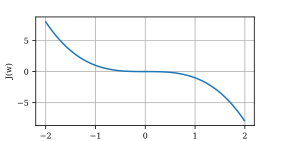
\includegraphics[scale=1]{Figures/Chapter_3/saddle_point.png}
	\end{center}
	\caption{Saddle point.} 
	\label{fig:saddle_point}
\end{figure}
%%%%%%%%%%%%%%%%%%%%%%%%%%%%%%%%%%%%%%%%%%%%%%%%%%%%%%%%%%%%%%%%%%%%%%%%%%%%%%%%
\subsection{Convolutional Neural Network} 
Convolutional Neural Networks (CNNs) are a special type of artificial neural network (ANN) that were initially developed in the 1980s by ~\textcite{Fukushima1980} who was inspired by the discoveries of Hubel and Wiesel regarding the cat's visual cortex. 
CNNs are one of the most utilised architectures in DL for image processing as they can recognise complex patterns of images by performing convolution operations.

In mathematics, a convolution is an operation performed between any two functions, as for example \(f, g:\mathbb{R}^{d} \to \mathbb{R}\) to produce at third function \((f\ast g)\) depicted in Eqn.~\ref{eqn:convolution}.
In which, we measure the overlap between \(f\) and \(g\), as one function is flipped and shifted by \(x\):
\begin{equation}
	(f\ast g)(x) = \int_{}^{} f(z)g(x-z)dz
	\label{eqn:convolution}
\end{equation}
In the case of discrete objects defined on the set \(\mathbb{Z}\) of integers, the integral operation turns into a summation of elementwise multiplied components, as depicted in Eqn.~\ref{eqn:discrete_conv}:
\begin{equation}		
	(f\ast g)(x) = \sum_{a}^{} f(a)g(i-a)
	\label{eqn:discrete_conv}
\end{equation}
For inputs with two dimensions, we have a corresponding sum with indices \((a,b)\) for \(f\) and \((i-a, j-b)\) for \(y\) respectively as depicted in Eqn.~\ref{eqn:2d_conv} that describes a cross correlation operation:
\begin{equation}
	(f\ast g)(i,j) = \sum_{a}^{}\sum_{b}^{}f(a,b)g(i-a,j-b)
	\label{eqn:2d_conv}
\end{equation}
%%%%%%%%%%%%%%%%%%%% from here
Convolution operation for image processing is essentially a cross-correlation operation also known as a sliding dot product or sliding inner-product. 
CNNs were designed to process data as tensors with different dimensions. 
For a 1D data tensor, it can represent various data forms, such as signals and sequences, in addition to sentences in various languages in translation problems.
For a 2D data tensor, it can represent an image in grayscale (one channel), further, by combining three 2D tensors a coloured 3D image is produced due to different intensities of the pixels in the (RGB) channels.
A 4D tensor represents volumetric data, such as a sequence of 3D images or a video.

A convolutional layer, has a number \( n\) of convolution kernels (filters), in  which,  each kernel has a set of weights, of a size \((w_k,h_k,d_k)\).
The kernel slides over an input image of a size \((w,h,d)\) performing a convolution operation (dot product), where \(w\) and \(h\) represent the image width and height, respectively, while \(d\) represents the depth (number of channels).
The output of the convolution operation are feature maps that are locally connected to the output of the previous layer. 
Figure~\ref{fig:convolution_3d} illustrates the convolution operation for a 3D input and the calculated output (feature map) with a new shape of \((h_{n}\times w_{n} \times d_{n})\).
%%%%%%%%%%%%%%%%%%%%%%%%%%%%%%%%%%%%%%%%%%%%%%%%%%%%%%%%%%%%%%%%%%%%%%%%%%%%%%%%
\begin{figure} [!ht]
	\begin{center}
		\centering
		\includegraphics[width=0.75\textwidth]{Figures/Chapter_3/convolution_operation_3D.png}
	\end{center}
	\caption{Convolution operation with a sliding kernel.} 
	\label{fig:convolution_3d}
\end{figure}
%%%%%%%%%%%%%%%%%%%%%%%%%%%%%%%%%%%%%%%%%%%%%%%%%%%%%%%%%%%%%%%%%%%%%%%%%%%%%%%%

Typically, the feature map size diminishes due to the convolution operation, though, the feature map can keep the same size of the input by applying some padding over the input. 
The calculations of new height and width of the output are illustrated in Eqns~\ref{new_hight} and~\ref{new_width}:
%%%%%%%%%%%%%%%%%%%%%%%%%%%%%%%%%%%%%%%%%%%%%%%%%%%%%%%%%%%%%%%%%%%%%%%%%%%%%%%
\begin{equation}
	h_{n} = \frac{h+2\times p-h_{k}}{s}+1
	\label{new_hight}
\end{equation}
%%%%%%%%%%%%%%%%%%%%%%%%%%%%%%%%%%%%%%%%%%%%%%%%%%%%%%%%%%%%%%%%%%%%%%%%%%%%%%%%
\begin{equation}
	w_{n} = \frac{w+2\times p-w_{k}}{s}+1.
	\label{new_width}
\end{equation} 
where \(h_{n}\) and \(w_{n}\) are the new height and width dimensions of the feature map respectively after applying the convolution. 
The padding \(p\) is added to the input image of a feature map to guarantee that both the input and the output have the same dimensions.
\(h_{k}\) and \(w_{k}\) represent the height and the width of the convolutional kernel, respectively.
The stride \(s\) defines how much the convolutional kernel slides each step during convolution.
The number of channels at the output feature map \((d_{n})\) equals the applied number of convolutional kernels \((n)\). 

Typically,  when we train a CNN model, its kernel weights are initialised randomly.
Accordingly, during the backpropagation process, all learnable parameters (kernels weights) are updated.
Consequently, kernels learn to detect different types of edges (vertical, horizontal, and diagonal edges), color intensities, etc.
%%%%%%%%%%%%%%%%%%%%%%%%%%%%%%%%%%%%%%%%%%%%%%%%%%%%%%%%%%%%%%%%%%%%%%%%%%%%%%%%

Commonly, a convolutional operation is followed by a non-linear activation function such as (relu, sigmoid, tanh), followed by a downsampling operation (pooling).
The idea behind pooling operation is to aggregate related features into one by reducing the spatial dimensions of the feature maps (e.g., width, height, and depth)~\cite{Lecun2015}, which reduces the computation complexity.
Figure~\ref{fig:downsampling} presents the downsampling operations that are max and average pooling, further, the pool size is \(2 \times 2\) with strides of \(2\).
The Maxpool picks the maximum value in the local pool filter in a feature map, whereas the average pool picks the average value in the local pool filter in a feature map.
%%%%%%%%%%%%%%%%%%%%%%%%%%%%%%%%%%%%%%%%%%%%%%%%%%%%%%%%%%%%%%%%%%%%%%%%%%%%%%%%
\begin{figure} [!ht]
	\begin{center}
		\centering
		\includegraphics[scale=1]{Figures/Chapter_3/downsampling.png}
	\end{center}
	\caption{Types of downsampling operations.} 
	\label{fig:downsampling}
\end{figure}
%%%%%%%%%%%%%%%%%%%%%%%%%%%%%%%%%%%%%%%%%%%%%%%%%%%%%%%%%%%%%%%%%%%%%%%%%%%%%%%%
A convolution operation, followed by a non-linear activation function, and pooling is referred to as a convolutional block.
Moreover, a convolutional block can be stacked and repeated several times. 
Finally, to pass the output from the convolutional block to the dense layer, a flattened layer is utilised to produce a 1D tensor.
Figure~\ref{fig:CNN} presents the default architecture of a CNN.
%%%%%%%%%%%%%%%%%%%%%%%%%%%%%%%%%%%%%%%%%%%%%%%%%%%%%%%%%%%%%%%%%%%%%%%%%%%%%%%%
\begin{figure} [!ht]
	\begin{center}
		\centering
		\includegraphics[width=1\textwidth]{Figures/Chapter_3/cnn.png}
	\end{center}
	\caption{Convolutional Neural Network architecture.} 
	\label{fig:CNN}
\end{figure}
%%%%%%%%%%%%%%%%%%%%%%%%%%%%%%%%%%%%%%%%%%%%%%%%%%%%%%%%%%%%%%%%%%%%%%%%%%%%%%%%

CNN became popular after the competition of the \enquote{Large Scale Visual Recognition Challenge 2012 (ILSVRC2012)}, when \textcite{Krizhevsky2012} introduced AlexNet~\cite{Krizhevsky2012}, which is a deep CNN applied on a large dataset of \(1,000,000\) images and \(1,000\) different classes.
AlexNet results were magnificent. 
The success has stimulated the progress of the development in GPUs technology and the use of the non-linear activation function Relu~\cite{Lecun2015}.
In the next years, several spectacular CNNs architectures were presented (e.g VGG-16, ResNet, Inception-v4, and others).
%%%%%%%%%%%%%%%%%%%%%%%%%%%%%%%%%%%%%%%%%%%%%%%%%%%%%%%%%%%%%%%%%%%%%%%%%%%%%%%%
\subsection{Recurrent neural networks}
\label{sec222}
Recurrent neural network (RNN) is a class of ANN that was introduced to work with time-series data (sequential data).
RNN technique can remember its data input, because of its internal memory, which makes it a powerful and promising technique in the field of DL.
Since there are temporal problems such as natural language processing, language translation, image captioning, and so on, they require to be handled sequentially.
In the traditional deep neural networks (feed-forward), the information only moves in one direction from the input layer through hidden layers to the output layers.
However, this is not the case for the RNN technique, which implies the current output of an RNN depends on the prior input sequence.
Accordingly, future events are also utilised for predicting the output of a given sequence.
Figure~\ref{fig:rnn_vs_FFNN} depicts the difference between RNN and feed-forward deep neural networks.
As shown in Fig.~\ref{fig:rrn}, for the RNN, the output of a certain layer is looped back to its input which helps in making the prediction.
However, in feed-forward networks shown in Fig.~\ref{fig:FFNN}, the inputs and outputs are independent, as there is only one direction for the data to move.
%%%%%%%%%%%%%%%%%%%%%%%%%%%%%%%%%%%%%%%%%%%%%%%%%%%%%%%%%%%%%%%%%%%%%%%%%%%%%%%%
\begin{figure}[!ht]
	\centering
	\begin{subfigure}{0.49\textwidth}		
		\centering
		\includegraphics[scale=1]{Figures/Chapter_3/recurrent_NN.png}
		\caption{} 
		\label{fig:rrn}
	\end{subfigure}
	\hfill
	\begin{subfigure}{0.49\textwidth}
		\centering
		\includegraphics[scale=1]{Figures/Chapter_3/feedforward_NN.png}
		\caption{} 
		\label{fig:FFNN}
	\end{subfigure}	
	\caption{(a) RNN v.s. (b) Feed-forward neural network.}
	\label{fig:rnn_vs_FFNN}
\end{figure}
%%%%%%%%%%%%%%%%%%%%%%%%%%%%%%%%%%%%%%%%%%%%%%%%%%%%%%%%%%%%%%%%%%%%%%%%%%%%%%%%

Figure~\ref{unrolled_rnn} presents a visualisation of an unrolled RNN, where \(x_{t}\) corresponds to the sequential timestamped input at time \(t\), \(h_{t}\) corresponds to internal state  and \(Y_{t}\) corresponds to the predicted timestamped output at time \(t\).
An unrolled RNN can be seen as a cascaded sequence of feed-forward networks.
%%%%%%%%%%%%%%%%%%%%%%%%%%%%%%%%%%%%%%%%%%%%%%%%%%%%%%%%%%%%%%%%%%%%%%%%%%%%%%%%
\begin{figure}
	\begin{center}
	\includegraphics[scale=1]{Figures/Chapter_3/unrolled_rnn.png}
	\end{center}
	\captionof{figure}{Unrolled RNN.}
	\label{unrolled_rnn}
\end{figure}
%%%%%%%%%%%%%%%%%%%%%%%%%%%%%%%%%%%%%%%%%%%%%%%%%%%%%%%%%%%%%%%%%%%%%%%%%%%%%%%%

In feed-forward neural networks, the learnable parameters (adjustable weights) are available only for the forward path of data propagation and are updated through the back-propagation algorithm.
In RNNs, there are two paths of data propagation (forward and backward). 
Hence, there are learnable weights for both directions.
Further, weights are updated using back-propagation through time (BBTT)~\cite{Werbos1990}.
BBTT depends on the number of timestamps, so it is computationally expensive when there are a high number of timestamps as BBTT performs a back-propagation algorithm on unrolled RNN.
Consequently, when implementing RNNs, issues may arise during updating the learnable weights using BBTT, which are vanishing and exploding gradients.
To overcome such issues, ~\textcite{Hochreiter1997} introduced a long short-term memory (LSTM), which is a memory extension for a regular RNN to address the problem of long-term dependencies.
Further, LSTMs handle inputs or outputs of any length, which makes LSTMs powerful for solving very complex sequential problems.
LSTM is composed of four units: an input gate, a cell state, a forget gate, and an output gate as presented in Fig.~\ref{fig:lstm}.
These gates help regulate the flow of information, which is added to or removed from the cell state. 
The hidden states in LSTM hold the short-term memory, while the cells state holds the long-term memory.
%%%%%%%%%%%%%%%%%%%%%%%%%%%%%%%%%%%%%%%%%%%%%%%%%%%%%%%%%%%%%%%%%%%%%%%%%%%%%%%%
\begin{figure}[h!]
	\begin{center}
		\includegraphics[scale=1]{Figures/Chapter_3/lstm.png}
	\end{center}
	\captionof{figure}{LSTM architecture.}
	\label{fig:lstm}
\end{figure}
%%%%%%%%%%%%%%%%%%%%%%%%%%%%%%%%%%%%%%%%%%%%%%%%%%%%%%%%%%%%%%%%%%%%%%%%%%%%%%%%

The purpose of the forget gate is to determine which information to consider and which to neglect.
The current input \(x_t\) and the previous hidden state \(h_{t-1}\) are passed through a sigmoid function which will produce values between \(0\) and \(1\).
Then the outputs of the sigmoid are multiplied with the previous cell state \(c_{t-1}\) to discard outputs equal to zero.
Equation~\ref{eqn:forget_gate} depicts the calculation at the forget gate:
%%%%%%%%%%%%%%%%%%%%%%%%%%%%%%%%%%%%%%%%%%%%%%%%%%%%%%%%%%%%%%%%%%%%%%%%%%%%%%%%
\begin{equation}
	\centering
	f_t = \sigma(W_f.[h_{t-1}, X_{t}]+ b_f),
	\label{eqn:forget_gate}
\end{equation}
%%%%%%%%%%%%%%%%%%%%%%%%%%%%%%%%%%%%%%%%%%%%%%%%%%%%%%%%%%%%%%%%%%%%%%%%%%%%%%%
where \(W\) represents the learnable weights, and \(b\) represents the bias term.

The input gate \(i_{t}\) takes the current input \(X_t\) with the previous hidden state \(h_{t-1}\) then apply the sigmoid function to get values in a range between 0 (not important) and 1 (important), then the
same current input \(X_t\), and the hidden state \(h_{t-1}\) are passed through a \(\tanh\) function at \(\tilde{C}_{t}\) that will regulate the network by transferring the values into a range between \(-1\) and \(1\).
Then, the outputs from the sigmoid and \(\tanh\) functions are multiplied point-by-point to eliminate \(0\) values.  
Equation~\ref{eq:eq2} depicts the calculation at the input gate:
\begin{equation}
	\begin{aligned}
		i_{t} &=\sigma\left(W_{i} \cdot\left[h_{t-1}, X_{t}\right]+b_{i}\right) ,
		\\
		\tilde{C}_{t} &=\tanh \left(W_{s} \cdot\left[h_{t-1}, X_{t}\right]+b_{c}\right).
	\end{aligned} \label{eq:eq2}
\end{equation}
At this point, the network has sufficient information obtained from the input and forget gates. 
Hence, the current cell state \(C_t\) is calculated by multiplying the previous cell state \(C_{t-1}\) with the output of the forget gate, then the result is added to the calculated input values as depicted in Eqn.~\ref{eq:eq3}:
\begin{equation}
	C_{t}=f_{t} * C_{t-1}+i_{t} * \tilde{C}_{t}.
	\label{eq:eq3}
\end{equation}
The output gate \(o_{t}\) computes the next hidden state \(h_{t}\) which
holds information related to the current inputs. 
Accordingly, the current input \(X_{t}\) and the previous hidden state \(h_{t-1}\) are passed through a third sigmoid function to produce values between \(0\) and \(1\).
The current cell state \(C_{t}\) is passed through a \(\tanh\) function and multiplied point-by-point with \(o_{t}\) to produce the new hidden state \(h_{t}\) which is transferred to the next timestamp.
Equation~(\ref{eq:eq4}) illustrates the calculations at the output gate:
%%%%%%%%%%%%%%%%%%%%%%%%%%%%%%%%%%%%%%%%%%%%%%%%%%%%%%%%%%%%%%%%%%%%%%%%%%%%%%%%
\begin{equation}
	\begin{aligned}
		o_{t} &=\sigma\left(W_{o}\left[h_{t-1}, X_{t}\right]+b_{o}\right),\\
		h_{t} &=o_{t} * \tanh \left(C_{t}\right).
	\end{aligned}
	\label{eq:eq4}
\end{equation} 
%%%%%%%%%%%%%%%%%%%%%%%%%%%%%%%%%%%%%%%%%%%%%%%%%%%%%%%%%%%%%%%%%%%%%%%%%%%%%%%%

Recently, LSTMs have been widely used for large-scale learning of language translation models, speech recognition systems, chatbots, forecasting stock markets, text data analysis, and many more~\cite{graves2014towards, cho2014properties}.
However, LSTMs are inefficient regarding capturing spatial information by themselves when the time series inputs are consecutive images.
Accordingly, the ConvLSTM layer, which is a combination of CNN and LSTM unit was introduced by Shi et al.~\cite{xingjian2015convolutional} to solve such a problem.
For ConvLSTM, the convolution operations are applied both at the input-to-state transition and at the state-to-state transitions.
ConvLSTM shown in Fig.~\ref{fig:ConvLSTM} is a variation of the LSTM cell as it performs a convolution operation within the LSTM cell.
%%%%%%%%%%%%%%%%%%%%%%%%%%%%%%%%%%%%%%%%%%%%%%%%%%%%%%%%%%%%%%%%%%%%%%%%%%%%%%%%
\begin{figure}[h!]
	\begin{center}
		\includegraphics[scale=1]{Figures/Chapter_3/convlstm_image.png}
	\end{center}
	\captionof{figure}{ConvLSTM architecture.}
	\label{fig:ConvLSTM}
\end{figure}
%%%%%%%%%%%%%%%%%%%%%%%%%%%%%%%%%%%%%%%%%%%%%%%%%%%%%%%%%%%%%%%%%%%%%%%%%%%%%%%%
ConvLSTM is a combination of a convolution operation and an LSTM cell.
Thus, ConvLSTM can capture the time-correlated and spatial features in a series of consecutive images. 
Equation~(\ref{eq:eq5}) depicts the ConvLSTM operations as the inputs \(X_1, \dots, X_t\), hidden states \(h_1, \dots, h_t\), cell states \(C_1, \dots, C_t\) and input, forget and output gates are represented as \(i_t, f_t\), and \(o_t\), respectively:
\begin{equation}
	\begin{aligned}
		i_{t} &=\sigma\left(W_{x i} * X_{t}+W_{h i} * h_{t-1}+W_{c i} \odot C_{t-1}+b_{i}\right) 
		\\
		f_{t} &=\sigma\left(W_{x f} * X_{t}+W_{h f} * h_{t-1}+W_{c f} \odot C_{t-1}+b_{f}\right) \\
		C_{t} &=f_{t} \odot C_{t-1}+i_{t} \odot \tanh \left(W_{x c} * X_{t}+W_{h c} * h_{t-1}+b_{c}\right) 
		\\
		o_{t} &=\sigma\left(W_{x o} * X_{t}+W_{h o} * h_{t-1}+W_{c o} \odot C_{t}+b_{o}\right) \\
		h_{t} &=o_{t} \odot \tanh \left(C_{t}\right)
	\end{aligned}
	\label{eq:eq5}
\end{equation}
where \(*\) indicates the convolution operation, and \(\odot\) represents the 
Hadamard product. 
Recently, ConvLSTM has become very popular and is increasingly being used in 
more and more image processing applications.
\section{Data-driven based SHM/NDT Techniques: Related work}
\label{sec33}
%%%%%%%%%%%%%%%%%%%%%%%%%%%%%%%%%%%%%%%%%%%%%%%%%%%%%%%%%%%%%%%%%%%%%%%%%%%%%%%%
The importance of SHM systems originates from their ability to monitor the condition of structures in real-time.
SHM systems can be developed using data-driven methods, which require a huge amount of data that are captured by monitoring the status of a structure.

The process of extracting features from structures in conventional techniques needs a lot of time and experts in the field.
Therefore, introducing machine learning methods to the feature extraction process became necessary.
Hence, deep learning methods can generalise and learn new features by themselves, which improves their functionality in damage estimation.

DL approach makes it possible to use registered data in their raw form without any need to perform feature extraction.
Hence, such an approach has an end-to-end structure that automatically learns and discovers the hidden features in a high dimensional input data~\cite{LeCun, Networks}.
Figure~\ref{fig:ML_vs_DL} illustrates the main differences between the conventional ML-based SHM and DL-based SHM approaches.

\begin{figure}[!ht]
	\centering
	\begin{subfigure}{1\textwidth}		
		\centering
		\includegraphics[width=1\textwidth]{Figures/Chapter_3/conventional_ML.png}
		\caption{} 
		\label{fig:ML_conventional}
	\end{subfigure}
	\\
	\begin{subfigure}{1\textwidth}
		\centering
		\includegraphics[width=1\textwidth]{Figures/Chapter_3/DL_approach.png}
		\caption{} 
		\label{fig:DL_approach}
	\end{subfigure}	
	\caption{(a) Conventional ML based SHM vs. (b) DL based SHM.}
	\label{fig:ML_vs_DL}
\end{figure}
%%%%%%%%%%%%%%%%%%%%%%%%%%%%%%%%%%%%%%%%%%%%%%%%%%%%%%%%%%%%%%%%%%%%%%%%%%%%%%%%
\textcite{Worden2007} have proposed several axioms related to SHM systems implemented using machine learning methods. 
According to them, damage detection can be perform\-ed in unsupervised learning.
However, recognising the damage type and how significant it is can not be performed without supervised learning. 
Moreover, the feature extraction process is essential for damage detection, and it can be performed by analysing and processing the signals captured by the sensors (e.g. PZT actuators), and then converting them to damage information.
Therefore, introducing machine learning methods to the feature extraction process became necessary.
Hence, machine learning methods can generalise and learn new features by themselves, which improves their functionality in damage estimation.

\subsection{Machine learning based SHM/NDT}
In recent years data-driven methods based on machine learning have increased in a significant way. 
In the following, I will present some methods for damage detection and estimation based on machine learning techniques.

%%%%%%%%%%%%%%%%%%%%%%%%%%%%PZT + SVM
\textcite{Das2010} presented a method for estimating several types of defects (delamination, saw cut, notches, and drilled holes) in composite material. 
For this purpose, a collection of PZT transducers were attached to the surface of the structure to generate and register Lamb waves propagation. 
Accordingly, a time-frequency domain was utilised to extract features related to defects from the registered response. 
Those extracted features were fed to one-class SVM, which performs classification and damage estimation. 
%%%%%%%%%%%%%%%%%%%%%%%%%%%% PZT + SVM

Moreover, \textcite{Dib2018} proposed a novelty classifier based on one-class SVM for detecting damage. 
The method was conducted by extracting data from damage impact on a glass-fibre composite plate and then evaluating the performance of the classifier. 
To extract the necessary features from the propagated wave the registered signal was segmented into L time bins, and the Fourier transform was applied to each time bin.
Accordingly, the features vector was constructed from the signal phase and the amplitude for each segmented time bin.
%%%%%%%%%%%%%%%%%%%%%%%%%%%%%%%%% PZT + PCA+ KNN + SVM

\textcite{Vitola2016} developed a damage detection and classification methodology that was examined on aluminium plates.
An array of PZT transducers was placed on the plate surface to sense wave propagation in the structure.
The methodology is based on the use of principal component analysis (PCA) and machine learning techniques for recognising patterns.
PCA means analysing a large amount of information by finding the principal components.
However, the PCA method is not invariant to scaling, thus, data must be normalized~\cite{Tibaduiza2016}.
Next, normalised data is fed to several machine learning models for training.
For this purpose, several classification algorithms were applied, decision trees, KNN and SVM.
However, only a few of these models presented good outputs in damage detection.

%%%%%%%%%%%%%%%%%%%%%%%%%%% KNN
\textcite{Godin2004} applied Acoustic Emission signals (AE) in their approach, which happen due to a sudden release of stored energy when damage occurs.
AE signals contain important information about the discriminative features 
for the damage type such as fibre breakage, de-cohesion of the interface, or a crack in the matrix in composite materials.
Authors in this work presented supervised and unsupervised classifiers to recognise different damage patterns through grouping AE signals from the tensile tests of unidirectional glass/polyester composite into several different classes. 
For clustering AE signals, a K-means algorithm was used. 
AE signals were clustered based on several metrics such as the AE signal duration, amplitude, rise time, and the number of counts to the peak.
Accordingly, the clustered labelled data is fed into a KNN supervised classifier.
A trained classifier can classify new coming data accordingly.
Regarding the unsupervised classification, the Kohonen classifier was utilised~\cite{58325}, which is a self-organising map (SOM) which is a neural network consisting of neurons as processing units. 

%%%%%%%%%%%%%%%%%%%%%%%%%%% 

\textcite{Nazarko2020} monitored the axial bolt forces using elastic wave propagation signals.
Six-bolt flange connections were put through a series of static tensile tests in the lab. 
For the accurate measurement of axial force, some bolts were equipped with washer load cells.
Additionally, a few bolts were equipped with piezoelectric transducers (actuator and sensor operating in a pitch-catch arrangement) to capture the elastic wave signals.
The outcomes of the ultrasonic testing were then integrated with the artificial neural network (ANN) for both signal compression and as a tool for user interface. 
The outcomes demonstrated that ANNs could predict the axial forces in bolts with a reasonable amount of accuracy. 
Significant potential exists for actual NDT inspections, according to the suggested method~\cite{Nazarko2020}. 

%%%%%%%%%%%%%%%%%%%%%%%%%%% KNN
\textcite{Pashmforoush2014} proposed a technique to classify damage to various lay-up configurations in glass/polyester composites.
For this purpose, the K-means algorithm with the genetic algorithm was utilised. 
PCA was used to reduce the data dimensionali\-ty.
Next, a combination of the K-means algorithm with the genetic algorithm is used for clustering the data. 
The reason for applying the genetic algorithm is to find the optimal number of cluster centres for the KNN algorithm.
Parameters of the AE signals such as peak amplitude, frequency, rise time, energy, and duration were estimated for each cluster and utilised as discriminative features. 
AE signal frequency was found to be a good feature for discrimination. Accordingly, AE signals with the highest frequency were corresponding to fibre breakage, AE signals with the lowest frequency were corresponding to matrix cracking, and the frequencies range in-between were corresponding to the debonding defect. 

%%%%%%%%%%%%%%%%%%%%%%%%%%%%%%%%%%%%%%%%%%%%%%%%%%%%%%%%%%%%%%%%
\textcite{Nazarko2016} investigated the potential of utilising artificially deteriorated signals of Lamb waves in training a novelty detection (ND) system for early damage detection.
To train auto-associative neural networks, the authors used principal components that were generated from signals that were measured experimentally.
The measurements of Lamb waves in the investigated specimens made of aluminium and glass fibre reinforced polymer serve as an excellent illustration of how the ND algorithm accurately handles both simple and complex signals.
It was also noted that the proposed ND method maintained its sensitivity and robustness when it used raw signals with a relatively low sampling rate, on a relatively narrow time window, and further noised signals.
%%%%%%%%%%%%%%%%%%%%%%%%%%%% PZT + ConvNet
%\textcite{Sammons2016} utilised X-ray computed tomography for estimating the delaminations in a CFRP. For this purpose, they utilised the Convolutional Network (ConvNet ) for performing image segmentation of the defected input images to estimate the delaminations. There ConvNet was capable of identifying  and quantifying small delaminations. 
%Unfortunately, the ConvNet could not recognise delaminations with large sizes.
%%%%%%%%%%%%%%%%%%%%%%%%%%%% PZT + ConvNet
%
%Moreover, \textcite{Chetwynd2008} have investigated curved carbon fibre composite panel for damage localisation. 
%Accordingly, stiffeners were used during the experiments to represent real-life damage. 
%For this purpose, authors attached a combination of PZT transducers on the panel used to generate and receive Lamb waves that propagate through the structure. 
%During their propagation through the structure, Lamb waves encounter defects, which affects their propagation response. 
%The collected response was transformed into a novel scaler index using outlier analysis~\cite{Beniger1980}, which was then fed to MLP. 
%The MLP used for classification and regression applications of damage detection. 
%Classification operation is responsible for predicting whether there is damage or not in a specific location. 
%Where the regression operation is responsible for the exact estimation of the damage location.
%%%%%%%%%%%%%%%%%%%%%%%%%%% Ful wavefield +ConvNets
%% SECTION HEADER ////////////////////////////////////////////////////////////////////////////////
\subsection{Deep learning based SHM/NDT}

Deep learning techniques have widely been utilised for the inspection and maintenance of civil infrastructure and have shown very promising results \cite{Cha2017b, Lin2017, liu2019computer, Beckman2019, Choi2020, Sonski2020a, Sonski2020, Sonski2019}. 

Besides the widespread applications of deep learning for SHM/NDT in civil engineering, deep learning is still less investigated for the purpose of damage detection based on guided waves in composite materials.

Guided waves approaches are widely utilised in SHM/NDT due to the fact it can detect very small damage sizes~\cite{Guemes2020}. 
Damage detection and localisation approaches using guided waves are based on the measurements of the PZT sensors, whether bonded or embedded into the investigated structure. 
PZT sensor(s) are responsible for the excitation of the structure by a short ultrasonic pulse (usually, the used frequency is in the range of hundreds of kHz) that propagates through an investigated structure such as plates or pipes as an elastic wave.
The registered signals (baseline) are stored and compared with other registered signals acquired through the lifetime of the investigated structure.
Damage detection using the baseline subtraction approach for guided waves is based on subtracting damage-free registered measurements from the newly registered measurements to obtain the new changes that occurred to the structure.
These changes are considered as damage information.
The baseline approach is effective in controlled environments where the variations of the operational/environments (i.e. considerations of multiple sensing modalities, uncertainty in material properties, bounding conditions, etc.) are negligible~\cite{Yuan2020}.  
Such variations can alter registered data leading to false alarms.
The effect of such variations can be reduced through physics-based modeling, which can simulate an undamaged scenario (baseline) for the wave propagation through the investigated structure.
Then, the simulated baseline can be used in the subtraction for damage detection.
However, in real-world structures, it is difficult to adjust the parameters of the model to match the experimental registered data.
Accordingly, data-driven techniques based on ML and DL approaches can be the solution and deliver robust models for many real-life variations.

In the following, methods for damage size estimation based on machine learning and deep learning techniques are presented, which are targeted in the field of SHM/NDT.

%\textcite{islam1994damage} presented one of the earliest research studies for assessing delamination location and size in composite structures using deep learning techniques.
%They trained a neural network model using frequencies from modal analysis data for the first five modes.
%Data were obtained using piezoceramic sensors in both damaged and undamaged composite beams.
%In the following, several approaches utilising guided waves for SHM/NDT based on data-driven techniques for damage detection and localisation are presented.

\textcite{Melville1949} proposed a CNN model for the prediction of damage state in thin metal plates to overcome the issue of inaccurate representation of guided wave propagation when applying conventional approaches. 
The model utilizes the full wavefie\-ld scans of thin plates (aluminium).
Moreover, the acquired raw data used for training the model was divided into undamaged and damaged states equally.
The model achieved higher accuracy regarding damage detection equal \(99.98\%\) when compared to SVM which achieved \(62\%\).

\textcite{Sammons2016} proposed a CNN model based on X-ray computed tomography for delamination estimation in a composite structure.
Furthermore, image segmentation was applied to the input images to identify the damage.
However, the model was only able to identify small delaminations.

Moreover,~\textcite{Chetwynd2008} presented a multi-layer perceptron (MLP) network for damage detection in curved composite panels, in which, stiffeners were added to represent the damage.
The Authors in this work investigated the propagation of Lamb waves through the panel in which they were generated and registered by a PZT array.
Furthermore, for each Lamb wave response, a novelty index was obtained.
The index value is compared to some threshold value, in which if the index value exceeds the threshold it implies that there is damage to the structure.
Accordingly, the MLP network was fed by obtained novelty indexes, and performed two operations: classification and regression.
The classification network was designed to define three convex regions of the panel and then to determine whether the panel is damaged or not.
On the other hand, the regression network is capable of estimating the exact location of the damage

Furthermore,~\textcite{DeFenza2015} proposed an artificial neural network (ANN) model for damage detection in plates made of aluminium alloys and composite utilising Lamb waves.
Response data of wave propagation were used to calculate damage indexes which were fed into the model as an input.
Accordingly, the model performs automatic feature extraction in conjunction with the probability ellipse-based method. 
The ANN model and probability ellipse (PE) method were applied to identify the damage location.
The results from the ANN model and the PE presents how it is useful to apply damage indexes as a baseline for such methods to evaluate damage in aluminium and composite structures. 
Ewald et al.~\cite{Ewald2019} presented a CNN model called (DeepSHM) for signal classification using Lamb waves.
Furthermore, the model provides an end-to-end approach for SHM by utilising response signals captured by sensors.
Moreover, response signals were preprocessed by wavelet transform to get the wavelet coefficient matrix (WCM).
Further, the CNN model was trained with the WCM to obtain neural weights.

Full wavefield scanning using SLDV is time-consuming, however, simply reducing the number of scanning points will result in low-quality images. 
\textcite{esfandabadideep} proposed a compressive Sensing technique using ConvNets to enhance the resolution for images captured by SLDV while decreasing the number of measurement scan points down to \(10\%\) of the number of the full gird scanning points. 
Although, the proposed technique enhanced the image resolution, however, there is a side effect, which resembles the fact when enhancing the resolution, the most affected region is the damaged area. 
Accordingly, the damage features will be altered.
On the other hand, this may be an indication of the location of the damage.

Furthermore,~\textcite{Melville2018} proposed a technique for damage detection in thin metal plates (aluminum and steel), using full wavefield data scanned by SLDV. 
Using this data to train a deep neural network of 4 hidden layers including 2 convolutional layers for features extraction and 2 fully connected layers. 
The developed model shown good results when compared with traditional machine learning SVM.
Moreover,~\textcite{Melville2017} introduced a method for detecting damage in structures based on the k-means algorithm. 
The method is known as~\enquote{dictionary learning} which uses full wavefield data collected from thin metal plates. 
The method was applied to structures with different material types and thicknesses that were not used during training to prove how well the model in damage detection in various conditions. 
However, their work was not implemented for a further step, which is damage localization and classification.

%\textcite{Ijjeh2021} presented a fully convolutional network (FCN)  for damage identification in composite plates base on a supervised learning approach.
%Furthermore, the authors utilised a full wavefield of Lamb waves propagation, which was numerically generated resembling measurements acquired by scanning laser Doppler vibrometer (SLDV).
%The model performs a pixel-wise segmentation that is able to identify the delamination which results in damaged and undamaged classes.
%Moreover, the model results were validated through a comparison with a conventional wavefield signal processing method i.e. adaptive wavenumber filtering~\cite{Radzienski2019,Kudela2018}.
%The proposed model achieved an accuracy of \(93.3\%\) in damage detection on numerical data compared to  \(64.8\%\) with the conventional method.
%Furthermore, the proposed model was verified on experimental data and it proved its ability for generalisation.
%%%%%%%%%%%%%%%%%%%%%%%%%%%%%%%%%%%%%%%%%%%%%%%%%%%%%%%%%%%%%%%%%%%%%%%%%%%%%%%%%%%%%%%%%%%%%%%%%%%%%%%%%%%%%%%%%%%%%%%%%%%%%%%%%%%%%%%%%%%%%%%%%%%%%%%%%%%%%%%%
%\subsection{Vibration based SHM though DL}
%\label{sec24}
%The vibration-based approach for damage assessment using ML techniques has been investigated thoroughly  for several SHM applications.
%Furthermore, introducing DL techniques for data-driven SHM applications has presented new scopes for investigating large scale structures and enhanced the process of data acquisition and processing of large datasets acquired by sensors of different types~\cite{Carden2004,Sohn1996}.
%Generally, the conventional approach for damage localisation requires prior knowledge of the approximate damage locations~\cite{Xu2018,Dorafshan2016}. 
%Therefore, the identification process regarding candidates for the damaged locations is complex and can consume plenty of time.
%Damage locations identification under the vibrational approach is based on the fact that the damage cause changes in the vibration characteristics such as modal shapes, frequencies, and damping~\cite{Doebling1998},
%which can be utilised in the identification of damaged locations from the registered data response of a structure.
%A vibration-based approach can be categorised into two classes:
%model-based (parametric) and non-model-based or (non-parametric).
%Parametric methods require computational models and associated assumptions about the investigated structure.
%In general parametric methods can achieve good accuracy, however, there is no guarantee regarding the availability of accurate information about the structural system in the real-world~\cite{Azimi2020}. 
%As a result, the non-parametric methods arise due to the challenges in developing robust computational models. 
%With non-parametric methods, there are no prior assumptions about the structural system.
%
%In the following, several vibration-based for SHM using DL techniques are presented.
%Authors in~\cite{Abdeljaber2017} introduced a damage identification approach based on output-only response data.
%In which, various damage cases (loose bolt) were investigated, accordingly training data were generated based on the acceleration response.
%Authors in this approach have trained several CNNs separately regarding each damage case, and accordingly, the probability of damage (PoD) was determined.
%By investigating scenarios of undamaged, single damage and multiple damage cases, they obtained \(0.54\%\) average error for specifically identified cases.
%
%Authors in~\cite{Lin2017} introduced a new approach to structural damage detection using CNN.
%Moreover, the authors have developed a numerical model of simply supported Euler Bernoulli beam.
%The detection model was designed to learn features and to identify damaged locations, moreover, it led to excellent results regarding the accuracy of damaged locations on the noise-free and noisy dataset.
%Wang and Cha in~\cite{Cha2018} proposed an unsupervised CNN model, that is able to extract the feature representations from the unlabelled data.
%The authors in their model used raw acceleration signals (sensitive to the damage presence) that were acquired from an intact lab-scale steel bridge.
%Then, the acquired response vector was normalised followed by applying the continuous wavelet transform (CWT) and fast Fourier transform (FFT).
%The output was then fed into a CNN auto-encoder,
%Accordingly, the extracted damage features were fed into one-class (OC) SVMs as novelty detectors corresponding to the sensors.
%Consequently, the approximation of damage location (loose-bolt) was estimated based on the locations of the sensors with the highest novelty rates.
%
%Motivated by human vision and thinking, authors in~\cite{Cha2018} presented a computer vision and deep-learning framework for anomaly detection.
%The proposed approach consists of two steps.
%In the first step, data conversion by data visualisation is carried out, in which it mimics human vision and thinking.
%In data visualisation,  the registered data response of acceleration is transformed into images plotted in gray-scale. 
%In the second step, the training dataset is labeled manually, then fed into deep convolutional neural networks (DCNNs).
%The proposed technique was tested on one-year data and achieved a global accuracy of \(87,0\%\) and it could be used for real-time SHM.
%Moreover, Tang et al. in~\cite{Tang2019} presented a DL technique for data anomaly detection which can be considered as an improved technique to the previous work in~\cite{Cha2018}.
%Initially, the raw time series measured data are split into segments, and data in the time and frequency domain are visualised. 
%Images related to each section are stacked as a single dual-channel (red and green).
%Then, the training dataset is fed into a CNN that learns how to perform data anomaly classification.
%The main difference between the previous approach and this approach was in using imbalanced data in which the number of samples of different classes was unequal, however, in this approach the used data were balanced.
%Finally, the comparison shows that this approach outperformed the previous one and achieved higher accuracy for all data anomaly patterns.
%
%Authors in~\cite{Wu2019} presented a study of the deep CNN method in estimating the dynamic response of a linear single-degree-of-freedom (SDOF) system, a nonlinear SDOF, and a multidegree of freedom (MDOF) streel frame.
%In some cases, the convolutional kernel can approximate the numerical integration operator, and the convolutional layer can be interpreted as a dominant frequency extraction operator.
%Moreover, different cases of noise-contaminated signals were investigated. 
%Additionally, MLP method was used as a reference to the proposed CNN approach.
%A comparison between the results obtained by the MLP and CNN shows that the CNN approach is more accurate and robust against noisy input data.
%
%Authors in ~\cite{Oh2019}  presented a study of the CNN technique for SHM application for response estimation of tall buildings under wind excitation.
%The proposed CNN model was trained on measured structural response data which take wind data measured as inputs in order to predict strains in future wind loads.
%In order to measure the performance of the proposed technique, it was verified with unseen data never used at the training phase and it was able to accurately estimate the maximum and minimum strains.
%Authors in~\cite{Li2020} proposed a CNN model for damage detection of a bridge structure.
%Moreover, the authors compared the performance of the CNN model with other techniques such as random forest, SVM, KNN, and decision tree, and the results showed that the accuracy was enhanced by at least \(15\%\).
%
%Since the acceleration response signal is highly prone to noise~\cite{Azimi2020}, researchers begin utilising other types of sensor data or use alternative features.  
%Li et al. in ~\cite{Li2020a} investigated damage in bridge structure accordingly, proposed a supervised learning technique based on the CNN model.
%Dataset was acquired by deflection of a scaled-down model bridge by a fibre-optic gyroscope.
%Then, the dataset was fed into a 1D-CNN model to classify three states of damage and an intact class (benchmark/damage-free).
%To investigate the performance of the proposed model, a cross-validation technique was applied. 
%It showed that the accuracy of the CNN model increased by at least \(15.3\%\) over other conventional methods such as SVM, KNN, decision trees, and random forests.
%Authors in \cite{Lopez-Pacheco2020} introduced a novel frequency-domain convolutional neural network (FDCNN) for damage detection based on Bouc-Wen hysteric model~\cite{Ismail2009}.  
%In the FDCNN method utilises only acceleration measurements for damage diagnosis, that are sensitive to environmental noise.
%Moreover, FDCNN reduces the computational time during the learning process, which increase noise robustness.
%The FDCNN introduced the spectral pooling operator responsible for attenuating the noise in measurements.
%The proposed method was validated through comparing it with different CNN model. 
%The performance of the proposed method was higher regarding damage identification in building structures.
%
%Finally, with smart monitoring as a target, authors in~\cite{Hung2020}  proposed a hybrid deep learning model for damage detection for SHM.
%The proposed model can deal with different damage levels and accurately detect damage by combining 1D-CNN and Long-Short Term Memory (LSTM) into a single end-to-end model fed by the raw time-series, and as a result, avoiding signal preprocessing step.
%Moreover, the proposed model verified that with low noise levels,  accurate damage detection can be achieved.
\section{Summary}
\label{sec34}
Moreover, author presented in this chapter several techniques that had studied and examined guided Lamb waves in composite materials to detect and localise the damage using signal processing techniques. 
Consequently, author concluded that those traditional techniques are complex and involve a huge numerical analysis and signal processing. Which concluded that the damage features are difficult to be extracted manually. 
Thus, new approaches that involve Machine and Deep Learning techniques are utilised are presented in this chapter. 
As a result, the process of damage features extracting became more convenient and easier since the machine is responsible for learning the new features and accordingly  detect and localise the damage. 
In consequence, it is concluded that the advantage of this approach is the improvement of feature damage extracting procedure.

Furthermore, problems with conventional damage detection techniques for SHM and the importance of the artificial intelligence approach were discussed.
Furthermore, in the second section of the chapter, the author introduced the ML approach in the SHM field.
Moreover, several techniques for feature extraction such as PCA, MSD, and GMMs were described. 
Further, several classification models such as SVM, KNN, and decision trees were introduced.
In the third section, DL approach was presented, in which techniques such as CNN  and RNN were presented.
Finally, several deep learning techniques for damage detection used regarding the SHM field based on guided waves and vibration approaches were presented.
%\input{Chapters/Chapter3/sect35}
%\input{Chapters/Chapter3/sect36}